\documentclass[../main.tex]{subfiles}

\subsection{Komponenten}
\begin{frame}
    \frametitle{IR-Spektrometer}
    \framesubtitle{Komponenten}
    \begin{columns}
        \column{0.5\textwidth}
        \begin{itemize}
            \item Strahlquelle
            \begin{itemize}
                \item Lötkolben
                \item $\lambda_{\text{max}} = \frac{b}{T} \approx \SI{7}{\micro\metre}$
            \end{itemize}
            \item Abblendende Optik
            \begin{itemize}
                \item Parabolspiegel
                \item Punktförmiger Strahl $\rightarrow$ Parallelstrahl
            \end{itemize}
            \item Optisches Gitter
            \begin{itemize}
                \item Gitter 100 Linien / mm
                \item $b_{100} \approx \SI{11}{\micro\metre}$
            \end{itemize}
            \item Sensor
        \end{itemize}
        \column{0.5\textwidth}
        \begin{figure}[ht]
            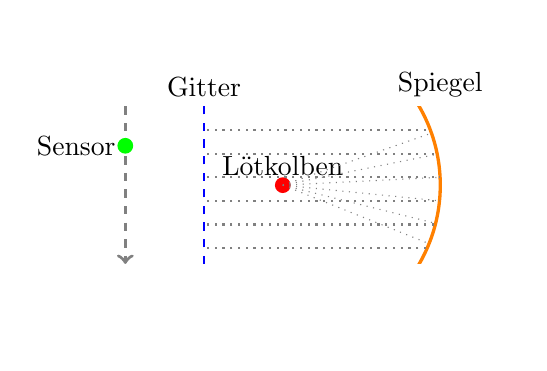
\begin{tikzpicture}
                % Spiegel
                \begin{scope}
                    \clip (2,1) rectangle (4,-1);
                    \draw (1,0)[orange,very thick] circle (2);
                \end{scope}
                \draw (3,1) node[black,anchor=south] {Spiegel};
                
                \fill[red] (1,0) circle (0.1) node[black,anchor=south] {Lötkolben};
                
                % EM-Strahlungen
                \begin{scope}
                    \clip (1,0) circle (2);
                    \clip (0,-1) rectangle (3,1);
                    \foreach \i in {0.3,0.6,...,2} {
                        \draw[gray,dotted] (1,0) -- (3,{\i-1.1}); % Abgegeben
                        \draw[gray,dotted,thick] (4,{\i-1.1}) -- (0,{\i-1.1}); % Reflektiert
                    }
                \end{scope}
                
                \draw[blue,thick,dashed] (0,-1) -- (0,1) node[black,anchor=south] {Gitter};
                
                \draw[very thick,gray,dashed,->] (-1,1) -- (-1,-1);
                \fill[green] (-1,0.5) circle (0.1cm) node[black,anchor=east] {Sensor};
            \end{tikzpicture}
            \caption{Schematischer Versuchsaufbau}
        \end{figure}
    \end{columns}
\end{frame}

\subsection{Versuch}
\begin{frame}
    \frametitle{IR-Spektrometer}
    \framesubtitle{Versuch}
    \begin{columns}
        \column{0.5\textwidth}
        \begin{itemize}
            \item 
        \end{itemize}
        \column{0.5\textwidth}
        \begin{figure}[ht]
            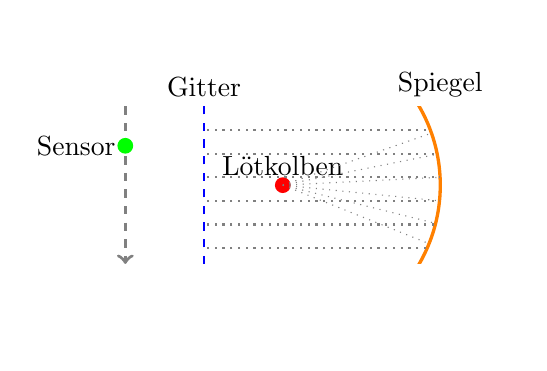
\begin{tikzpicture}
                % Spiegel
                \begin{scope}
                    \clip (2,1) rectangle (4,-1);
                    \draw (1,0)[orange,very thick] circle (2);
                \end{scope}
                \draw (3,1) node[black,anchor=south] {Spiegel};
                
                \fill[red] (1,0) circle (0.1) node[black,anchor=south] {Lötkolben};
                
                % EM-Strahlungen
                \begin{scope}
                    \clip (1,0) circle (2);
                    \clip (0,-1) rectangle (3,1);
                    \foreach \i in {0.3,0.6,...,2} {
                        \draw[gray,dotted] (1,0) -- (3,{\i-1.1}); % Abgegeben
                        \draw[gray,dotted,thick] (4,{\i-1.1}) -- (0,{\i-1.1}); % Reflektiert
                    }
                \end{scope}
                
                \draw[blue,thick,dashed] (0,-1) -- (0,1) node[black,anchor=south] {Gitter};
                
                \draw[very thick,gray,dashed,->] (-1,1) -- (-1,-1);
                \fill[green] (-1,0.5) circle (0.1cm) node[black,anchor=east] {Sensor};
            \end{tikzpicture}
            \caption{Schematischer Versuchsaufbau}
        \end{figure}
    \end{columns}
\end{frame}

\subsection{Arduino}
\begin{frame}
    \frametitle{IR-Spektrometer}
    \framesubtitle{Arduino}
\end{frame}
